%!TEX root = ../template.tex
%%%%%%%%%%%%%%%%%%%%%%%%%%%%%%%%%%%%%%%%%%%%%%%%%%%%%%%%%%%%%%%%%%%%
%% 4-Work_Done.tex
%% NOVA thesis document file
%%
%% Chapter with the template manual
%%%%%%%%%%%%%%%%%%%%%%%%%%%%%%%%%%%%%%%%%%%%%%%%%%%%%%%%%%%%%%%%%%%%

\typeout{NT FILE 4-Work_Done.tex}%

\chapter{Developed Work}
\label{cha:Developed Work}

\glsresetall

\section{Introduction} \label{sec.4:Introduction}
As discussed in Section~\ref{cha:State of the art}, most existing methods for agent separation and encirclement operate either in \gls{2D} or \gls{3D}. This chapter focuses on a method that is believed to differ from those previously presented for \gls{3D} formations. While it builds upon them as a basis and source of inspiration, it introduces a novel approach to separation on the two-sphere.

This chapter is structured into two principal components. The first concerns methods for distributing points on the two-sphere (Section~\ref{sec.4:Comparison of Agent Distributions on the Two-Sphere}), addressing how the desired final positions of a given number of agents can be arranged over the sphere. The second component presents the outer-inner control-loop architecture (Section~\ref{sec.4:Control loop architecture}), detailing both the outer agent controller and the inner controller responsible for the motion of points on the sphere.

\section{Comparison of Agent Distributions on the Two-Sphere} \label{sec.4:Comparison of Agent Distributions on the Two-Sphere}

As outlined in Section~\ref{sec.3:Agent spacing on the two-sphere}, multiple approaches exist for distributing a prescribed number of agents on the two-sphere. In this section, the outcomes of each method are presented and systematically compared. Based on this comparison, the most suitable method is identified in light of the objectives and constraints of the present study.

\begin{figure}[htbp]
\centering

\begin{minipage}{0.12\textwidth} % width for the row label
Latitude and\\Longitude:
\end{minipage}%
\begin{minipage}{0.85\textwidth} % width for the row of sub figures
\subfloat[Normal]{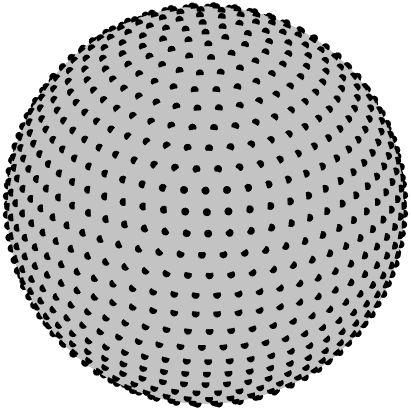
\includegraphics[width=3cm]{5-Figures/Chapter4/latlon_sphere/latlon_sphere_normal.png}}\hfil
\subfloat[Top]{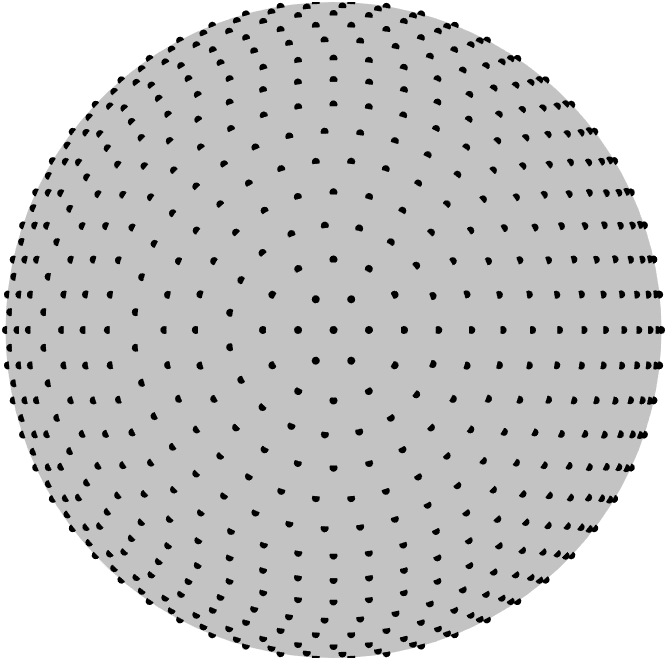
\includegraphics[width=3cm]{5-Figures/Chapter4/latlon_sphere/latlon_sphere_top.png}}\hfil 
\subfloat[Side]{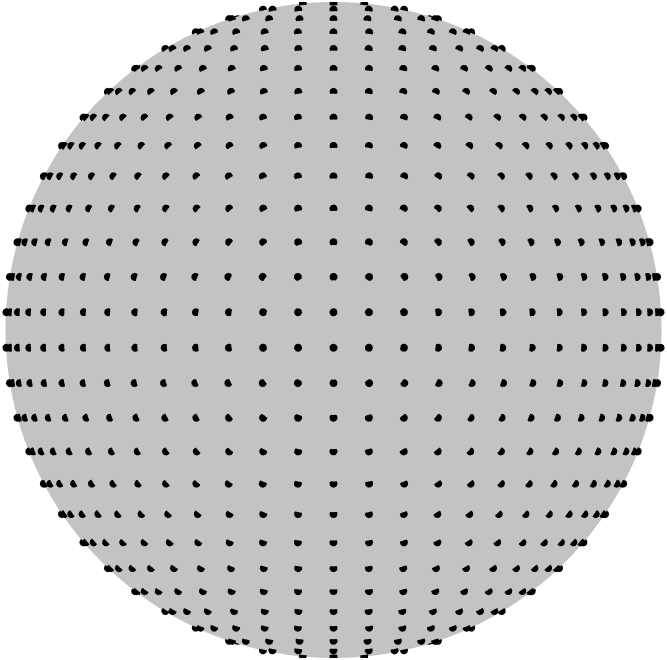
\includegraphics[width=3cm]{5-Figures/Chapter4/latlon_sphere/latlon_sphere_side.png}}
\end{minipage}

\vspace{0.3cm}

\begin{minipage}{0.12\textwidth}
Fibonacci\\Lattice:
\end{minipage}%
\begin{minipage}{0.85\textwidth}
\subfloat[Normal]{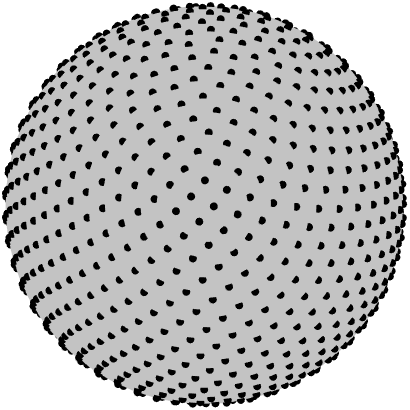
\includegraphics[width=3cm]{5-Figures/Chapter4/fibonacci_sphere/fibonacci_sphere_normal.png}}\hfil   
\subfloat[Top]{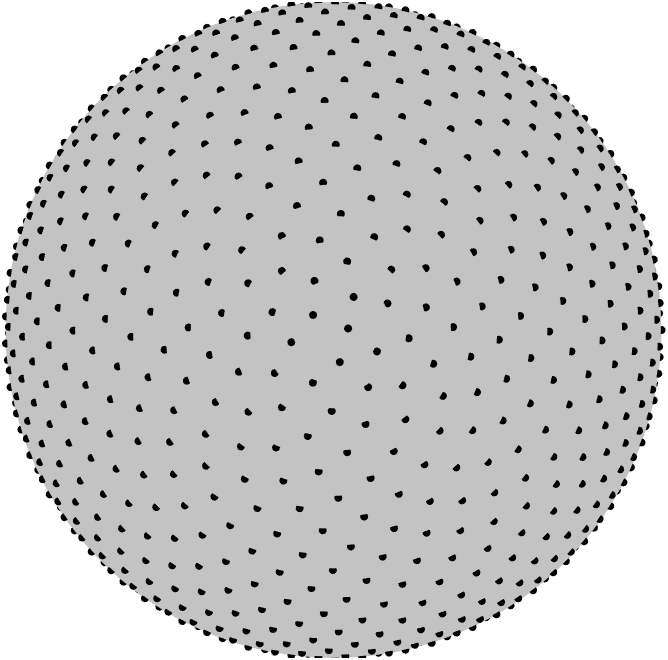
\includegraphics[width=3cm]{5-Figures/Chapter4/fibonacci_sphere/fibonacci_sphere_top.png}}\hfil
\subfloat[Side]{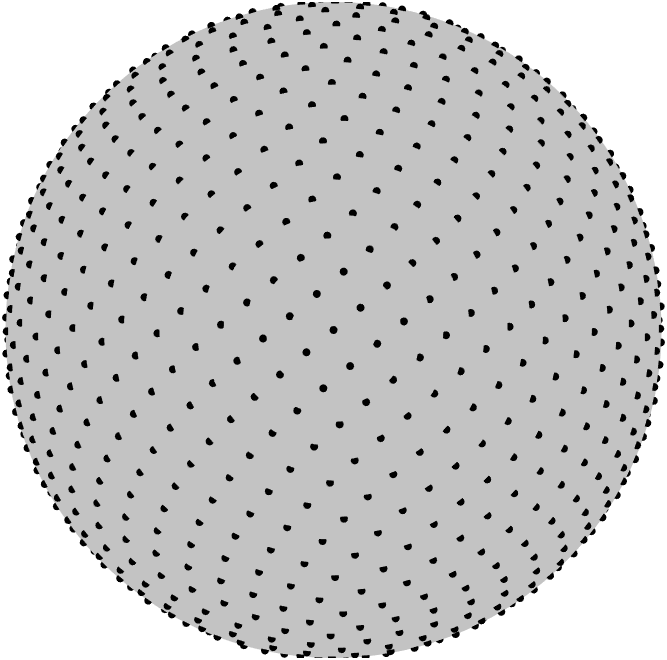
\includegraphics[width=3cm]{5-Figures/Chapter4/fibonacci_sphere/fibonacci_sphere_side.png}}
\end{minipage}

\vspace{0.3cm}

\begin{minipage}{0.12\textwidth}
Thomson\\Minimal Energy:
\end{minipage}%
\begin{minipage}{0.85\textwidth}
\subfloat[Normal]{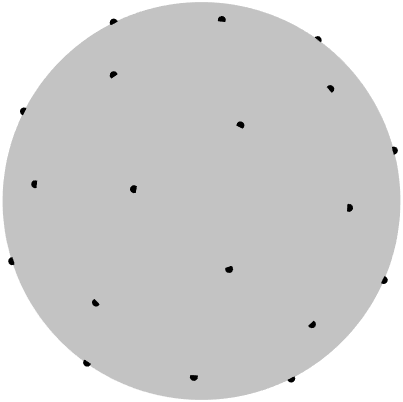
\includegraphics[width=3cm]{5-Figures/Chapter4/thomson_sphere/thomson_normal.png}}\hfil   
\subfloat[Top]{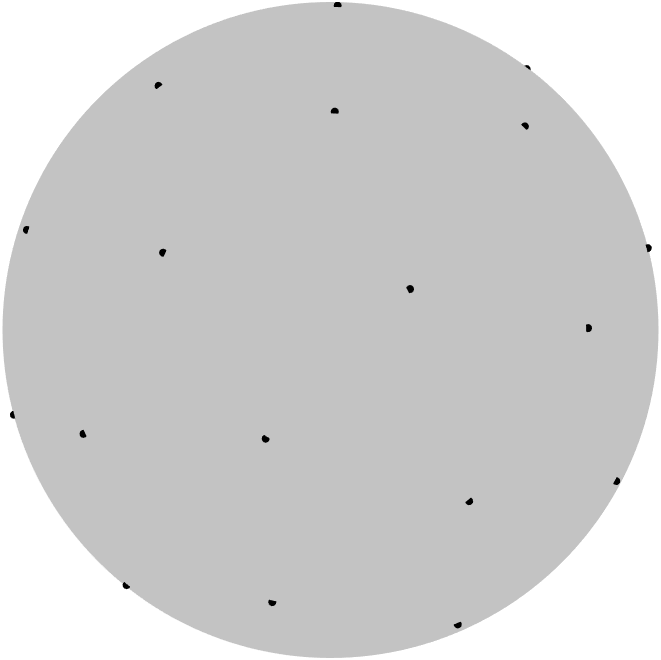
\includegraphics[width=3cm]{5-Figures/Chapter4/thomson_sphere/thomson_top.png}}\hfil
\subfloat[Side]{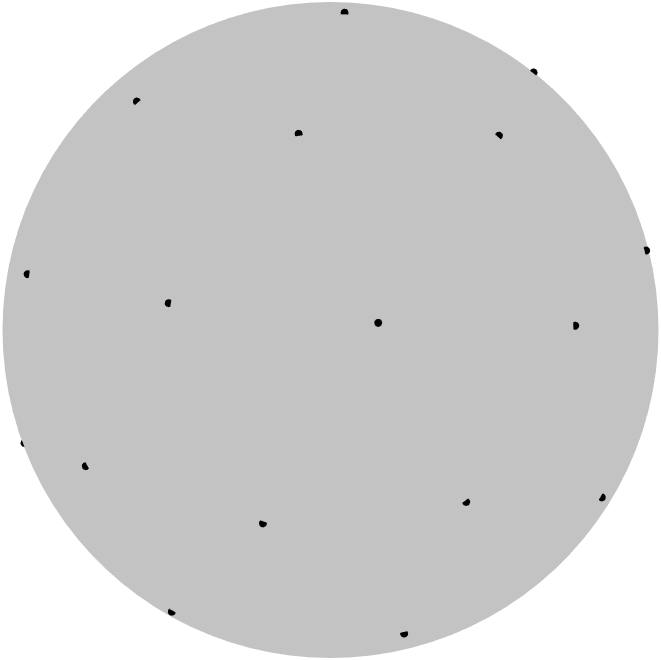
\includegraphics[width=3cm]{5-Figures/Chapter4/thomson_sphere/thomson_side.png}}
\end{minipage}

\vspace{0.3cm}

\begin{minipage}{0.12\textwidth}
Poisson Disk\\Sampling:
\end{minipage}%
\begin{minipage}{0.85\textwidth}
\centering
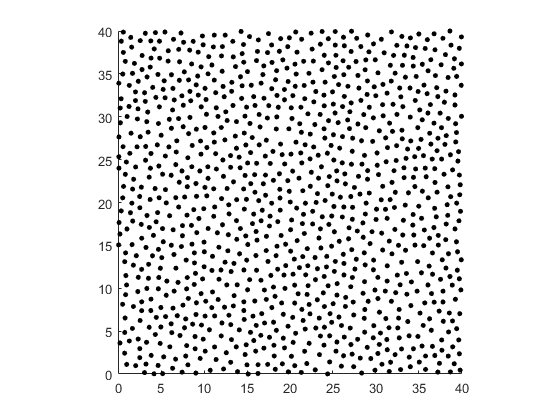
\includegraphics[width=5cm]{5-Figures/Chapter4/poisson_disk_sampling.png}
\end{minipage}

\caption{Agent positions resulting from each distribution methods.}
\label{fig.4:methods_points_on_sphere}
\end{figure}

\begin{figure}[htbp]
  \centering
  \captionsetup{justification=centering,margin=2cm}

  \begin{minipage}[t]{0.48\textwidth}
    \centering
    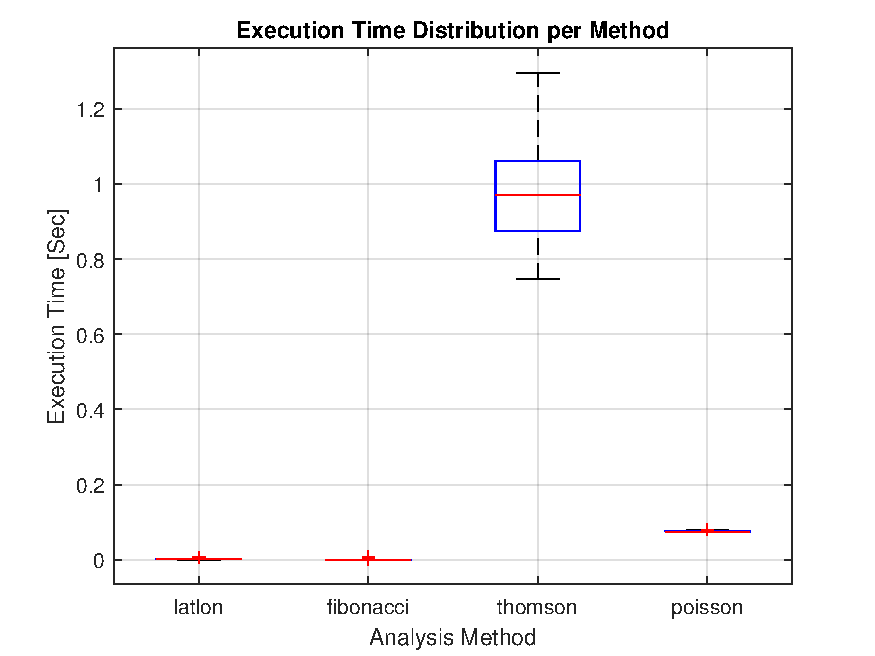
\includegraphics[width=\textwidth]{5-Figures/Chapter4/comparing_methods_box_shape.pdf}
    
  \end{minipage}
  \hfill
  \begin{minipage}[t]{0.48\textwidth}
    \centering
    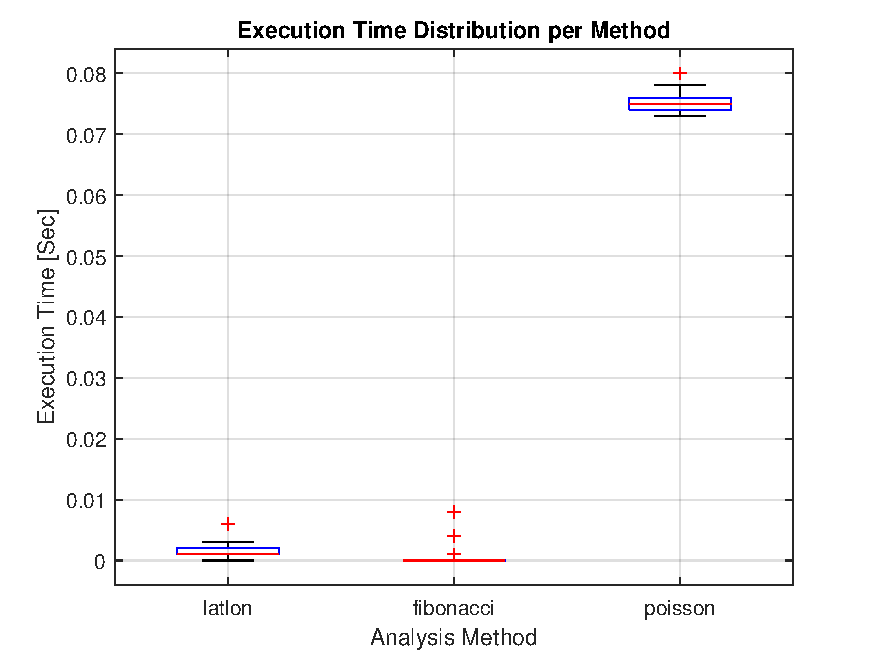
\includegraphics[width=\textwidth]{5-Figures/Chapter4/comparing_methods_box_shape_2.pdf}
  \end{minipage}
  \caption{Overall runtime comparison of the different methods (100 trials). Computer specification can be found at: \ref{appendix:Computer Specifications}}
  \label{fig.4:comparing_methods_box_shape}
\end{figure}


As shown in Figures~\ref{fig.4:methods_points_on_sphere}, the four methods produce noticeably different agent distributions. The longitude \& latitude method can be discarded due to its highly non-uniform spacing, which results in clustering near the poles as well as the limitation of number of agents. Thomson's minimal energy method, while producing high-quality uniform distributions, is much more computationally expensive then the others methods as can be seen in Figure~\ref{fig.4:comparing_methods_box_shape} and Table~\ref{tab.4:Runtime comparison of point sampling methods}, the average time is 0.9753 while the others are at least 10x faster (between $2.4 \times 10^{-4}$  and $0.0751$) and therefore, impractical for larger numbers of agents (note that only 31 agents where being used) compared with the 1000 plus of the other methods.



\begin{table}[htbp]
\caption{Runtime comparison of point sampling methods}
\label{tab.4:Runtime comparison of point sampling methods}
\centering
\begin{tabular}{l c c c c}
\hline
\textbf{Property}
& \makecell{\textbf{Lon--Lat}}
& \makecell{\textbf{Fibonacci}}
& \makecell{\textbf{Thomson}}
& \makecell{\textbf{Poisson Disk}} \\
\hline
\makecell{Parameters}
& \makecell{$K=29$}
& \makecell{--}
& \makecell{MaxIter=20000,\\ Seeds=1--100}
& \makecell{$40\times40$,\\ $r=1$} \\

\makecell{Number of points}
& \makecell{1070}
& \makecell{1001}
& \makecell{31}
& \makecell{1028} \\

\makecell{Mean runtime\\ (s)}
& \makecell{0.0016}
& \makecell{$2.4\times10^{-4}$}
& \makecell{0.9753}
& \makecell{0.0751} \\

\makecell{Std. deviation\\ $\sigma$ (s)}
& \makecell{$7.6877\times10^{-4}$}
& \makecell{$9.3333\times10^{-4}$}
& \makecell{0.1169}
& \makecell{0.0014} \\
\hline
\end{tabular}
\end{table}

This leaves two viable options: the Fibonacci lattice and Poisson disk sampling. The Fibonacci lattice is the fastest of the two methods as shown in Figure~\ref{fig.4:comparing_methods_box_shape} being still $666.66\dots\%$ faster on average while providing uniform coverage, but it is restricted to distributions on a spherical surface and is less flexible for arbitrary domains. Poisson disk sampling, in contrast, is more versatile and can be applied to arbitrary geometries, but it requires more computation and a gradient-based refinement step to achieve a fixed number of agents being the necessary separation distance initially unknown. Each method thus presents a trade-off between computational efficiency, uniformity, and flexibility. Due to the simplicity of the Fibonacci Lattice, it was chosen at the current time but with the development of the research it may be possible to generalize into any manifold making then necessary the transition to the Poisson Disk sampling.

\section{Alternative Agent Positioning Strategies} \label{sec.4:Alternative Agent Positioning Strategies}

This section discusses alternative methods that were considered to work to position agents on a spherical surface. Although the final configuration of each drone is based on the Fibonacci lattice, several other approaches were investigated, inspired by phase-separation methods commonly used for 2D formations \cite{Litimein2021}, \cite{Jin2018}, \cite{Kim2007}.  In particular, an attempt was made to develop a displacement-based 3D method in which each drone maintains a fixed angular separation from its predecessor.

The standard Fibonacci lattice formulation could not be directly applied in this context. While the longitude increments between agents are constant, allowing a simple angular separation rule, the latitude is computed through a nonlinear $\arcsin(\cdot)$ mapping, which is inherently non-uniform. This nonlinearity prevents the use of a single, constant spacing rule across all agents. Several attempts were made to linearize this relationship so that all agents could rely on identical local control laws, but none yielded satisfactory results. For completeness, the tested approaches are summarized below.

\subsection{Mean Distance Between Points on the Sphere}
In the first attempt, the geodesic distance between consecutive agents in the sequence was computed, and the mean of these distances was used as a reference spacing. This approach proved unsuccessful, as illustrated in Figure~\ref{fig.4:fibonacci_diff_methods} (row~2). The mean distance is heavily skewed by agents located near $\theta = \pi$, where inter-agent distances are significantly larger. For example, with 1001 points distributed on a sphere of radius $R = 5$, the mean distance was approximately 7.3270, corresponding to more than half the sphere's diameter. As a result, this metric does not provide a meaningful or usable spacing reference.

\subsection{Mean Latitude Spacing}
Since the primary source of nonlinearity lies in the latitude distribution, a second approach considered using the average latitude increment instead of the $\arcsin(\cdot)$ mapping. However, this method introduces a different issue: the geodesic distance between agents increases as the effective radius of the latitude circle grows, particularly near $\theta = \pi$. This results in a pronounced clustering of points near longitudes $\phi = 0$ and $\phi = 2\pi$, as shown in Figure~\ref{fig.4:fibonacci_diff_methods} (row~3). While the $\arcsin(\cdot)$ formulation avoids this clustering, the mean-latitude approach fails to preserve uniform surface spacing.

\subsection{Linearized Vertical Distribution with Uniform Angular Progression}
A final attempt aimed to mitigate the clustering near the poles by enforcing a uniform angular progression while simultaneously liberalizing the vertical distribution. Instead of relying on the nonlinear Fibonacci latitude mapping, a constant latitude increment $\theta_{\text{mean}} = \pi / P$ was imposed. In parallel, a constant longitude increment $\phi_{\text{mean}}$ was computed from the average difference of the Fibonacci-based longitudes.

The Cartesian coordinates of each agent were defined as
\begin{equation}
x_i = R \sin(i\theta_{\text{mean}})\cos(i\phi_{\text{mean}}), \quad
y_i = R \sin(i\theta_{\text{mean}})\sin(i\phi_{\text{mean}}),
\end{equation}
with the vertical coordinate distributed linearly according to
\begin{equation}
z_i = -R + \frac{R}{P} + \frac{2R(i-1)}{P},
\end{equation}
thereby enforcing equal spacing along the $z$-axis.

The motivation for this approach was twofold. First, by fixing $\theta_{\text{mean}}$, each agent would only need to maintain a constant angular separation from its predecessor. Second, by distributing agents uniformly along the vertical axis, the excessive clustering near the poles observed in previous methods could be reduced. As shown in Figure~\ref{fig.4:fibonacci_diff_methods} (row~4), this method successfully eliminates severe polar clustering and yields a visually more homogeneous vertical distribution.

However, despite these improvements, this approach still fails to guarantee uniform geodesic distances between neighboring agents. The imposed linearity in both $\theta$ and $z$ conflicts with the intrinsic geometry of the sphere, resulting in distorted inter-agent spacing. In particular, agents near the north and south region become closer than desired. The resulting shape comes due to the fact the points are forced (as intended) to spread equally along the z axis but this in turn makes the $i^{th}$ element be much lower than would be expected by X and Y coordinates.

\begin{figure}[htbp]
\centering

\begin{minipage}{0.12\textwidth}
Fibonacci\\Lattice:
\end{minipage}%
\begin{minipage}{0.85\textwidth}
\subfloat[Normal]{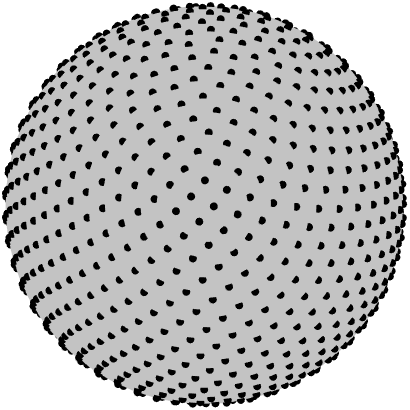
\includegraphics[width=3cm]{5-Figures/Chapter4/fibonacci_sphere/fibonacci_sphere_normal.png}}\hfil   
\subfloat[Top]{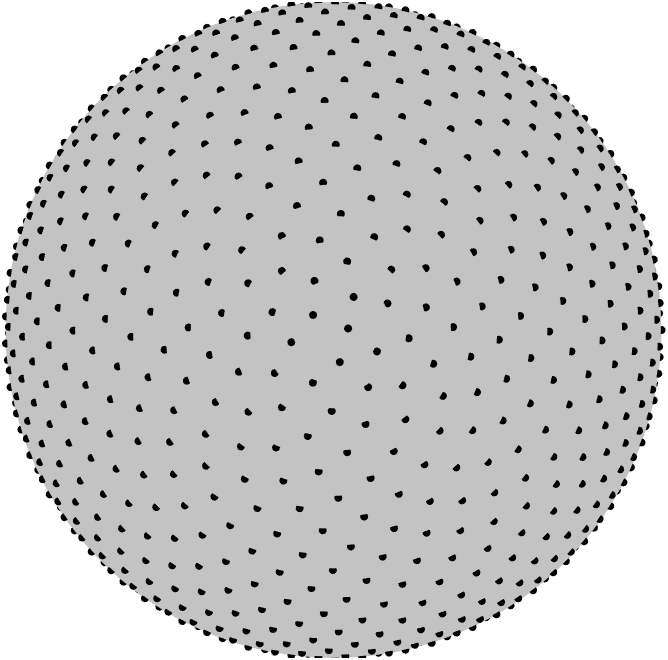
\includegraphics[width=3cm]{5-Figures/Chapter4/fibonacci_sphere/fibonacci_sphere_top.png}}\hfil
\subfloat[Side]{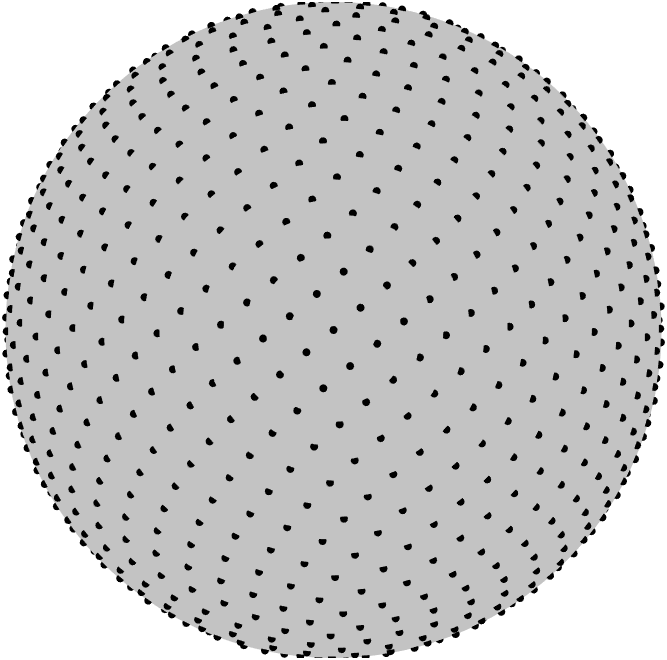
\includegraphics[width=3cm]{5-Figures/Chapter4/fibonacci_sphere/fibonacci_sphere_side.png}}
\end{minipage}

\vspace{0.3cm}

\begin{minipage}{0.12\textwidth}
mean\\dist:
\end{minipage}%
\begin{minipage}{0.85\textwidth}
\subfloat[Normal]{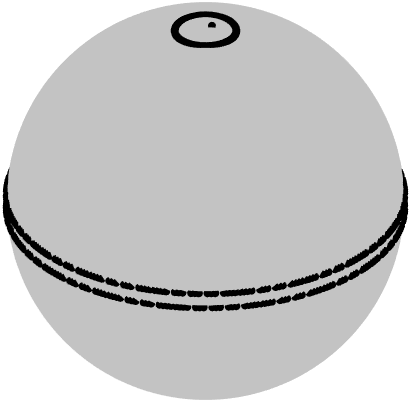
\includegraphics[width=3cm]{5-Figures/Chapter4/fibonacci_sphere_mean_dist/fibonacci_sphere_mean_dist_normal.png}}\hfil   
\subfloat[Top]{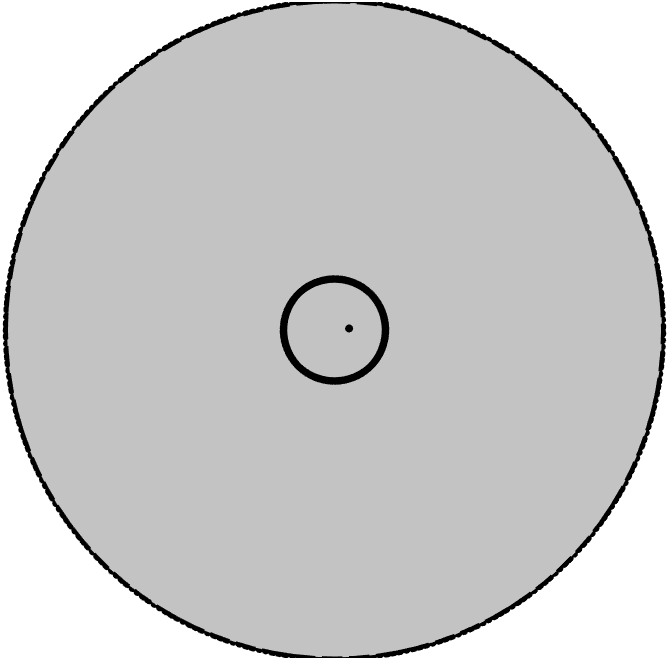
\includegraphics[width=3cm]{5-Figures/Chapter4/fibonacci_sphere_mean_dist/fibonacci_sphere_mean_dist_top.png}}\hfil
\subfloat[Side]{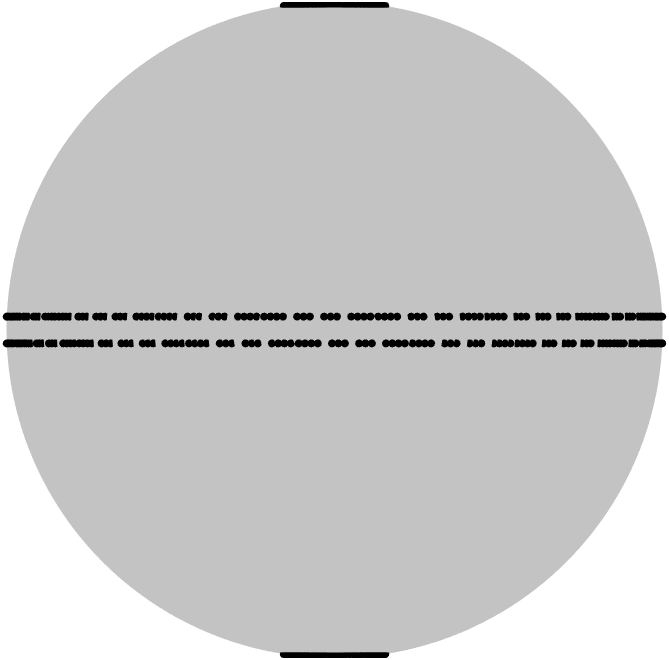
\includegraphics[width=3cm]{5-Figures/Chapter4/fibonacci_sphere_mean_dist/fibonacci_sphere_mean_dist_side.png}}
\end{minipage}

\vspace{0.3cm}

\begin{minipage}{0.12\textwidth}
mean theta:
\end{minipage}%
\begin{minipage}{0.85\textwidth}
\subfloat[Normal]{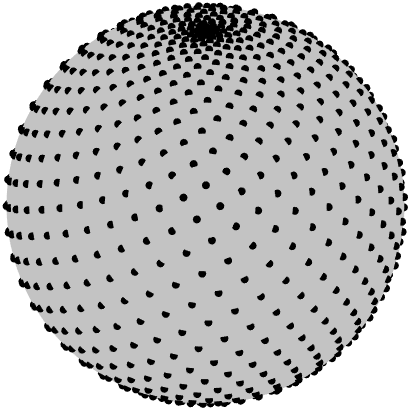
\includegraphics[width=3cm]{5-Figures/Chapter4/fibonacci_sphere_mean_theta/fibonacci_sphere_mean_theta_normal.png}}\hfil   
\subfloat[Top]{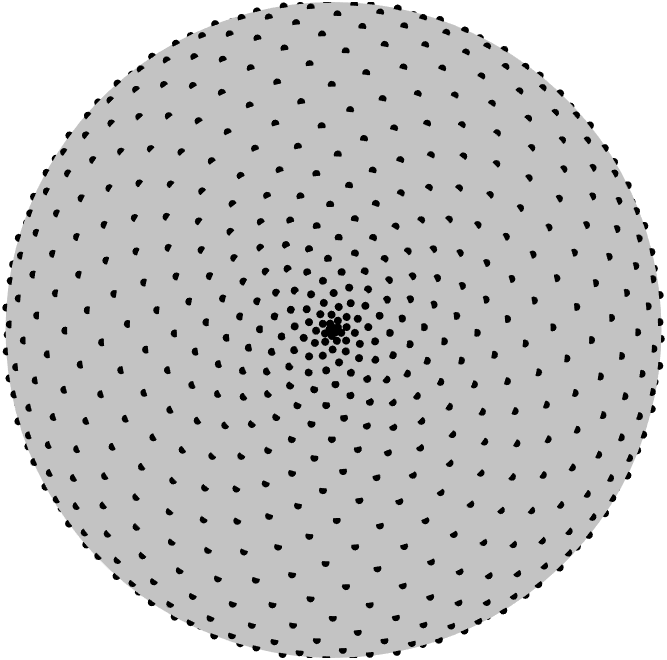
\includegraphics[width=3cm]{5-Figures/Chapter4/fibonacci_sphere_mean_theta/fibonacci_sphere_mean_theta_top.png}}\hfil
\subfloat[Side]{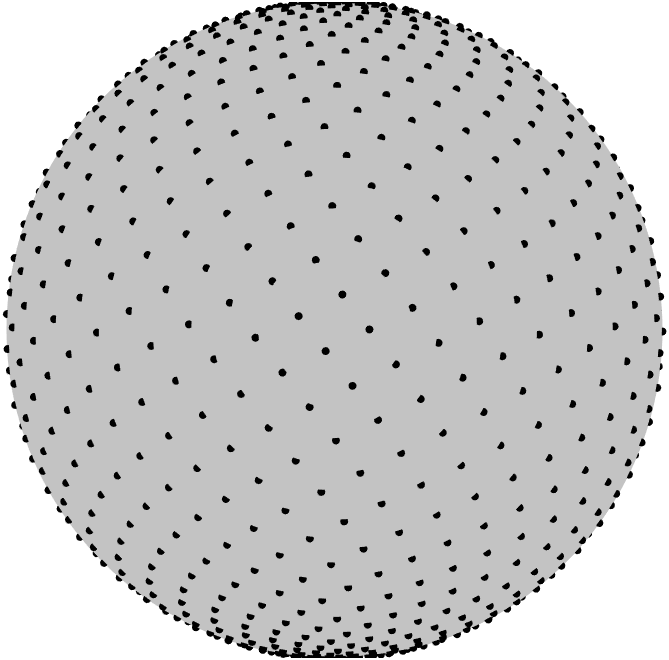
\includegraphics[width=3cm]{5-Figures/Chapter4/fibonacci_sphere_mean_theta/fibonacci_sphere_mean_theta_side.png}}
\end{minipage}

\vspace{0.3cm}
\begin{minipage}{0.12\textwidth}
mean theta\\eq z:
\end{minipage}%
\begin{minipage}{0.85\textwidth}
\subfloat[Normal]{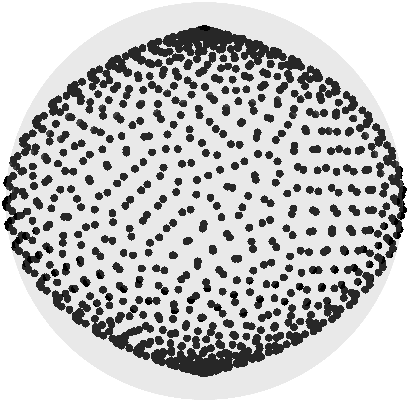
\includegraphics[width=3cm]{5-Figures/Chapter4/fibonacci_sphere_mean_theta_eq_z/fibonacci_sphere_mean_theta_eq_z_normal.png}}\hfil   
\subfloat[Top]{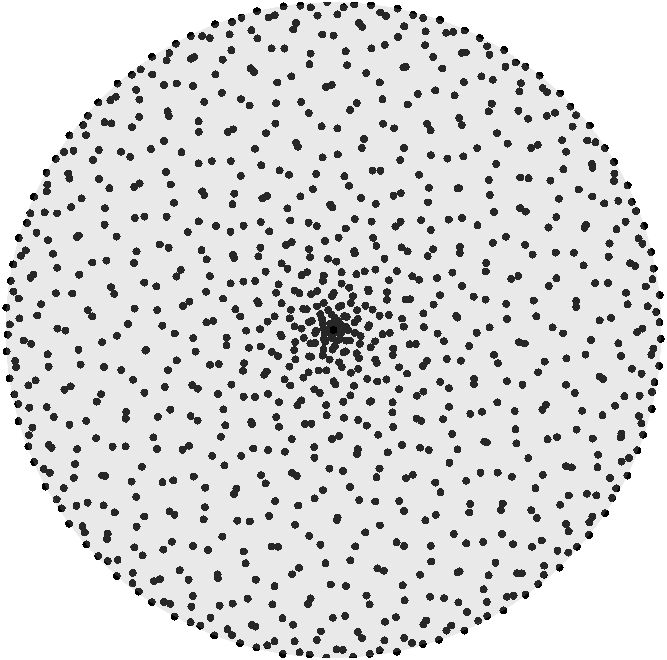
\includegraphics[width=3cm]{5-Figures/Chapter4/fibonacci_sphere_mean_theta_eq_z/fibonacci_sphere_mean_theta_eq_z_top.png}}\hfil
\subfloat[Side]{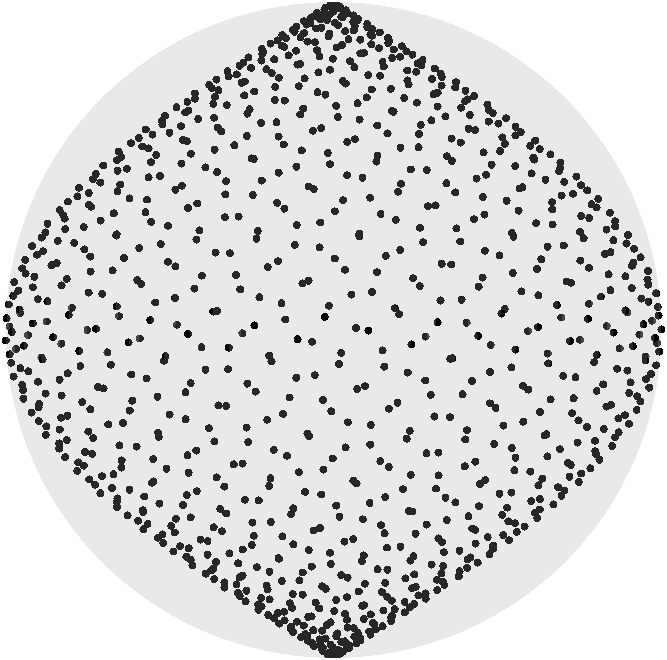
\includegraphics[width=3cm]{5-Figures/Chapter4/fibonacci_sphere_mean_theta_eq_z/fibonacci_sphere_mean_theta_eq_z_side.png}}
\end{minipage}
\caption{Different linearization of fibonacci lattice}
\label{fig.4:fibonacci_diff_methods}
\end{figure}

In summary, while this final approach partially alleviates the pole-clustering problem and simplifies the local control law by enforcing constant angular steps, it does so at the cost of losing the equal-area and near-uniform spacing properties of the standard Fibonacci lattice. As a result, it was ultimately deemed unsuitable for the final deployment strategy, but is included here for completeness and comparison with the other attempted methods. Either way this approach was flawed since opposite of the 2D approach where all drones are keeping a distance from the previous and next, in 3D the "top" and "bottom" drones aren't associated in any away.


\section{Control loop architecture} \label{sec.4:Control loop architecture}

This section focuses on how was the control of the drone in this case a quadrotor implemented in order to not only have the drone go to a desired position but also never collide with other agents. The system can be, as mentioned in the introduction, separated in two loops the inner loop responsible for having the actuation on the drone go to a desired waypoint with a desired velocity accelerations angle etc, as well as an outer loop that moves the drones desired waypoint, \gls{q},to the final desired point on the two-sphere, \gls{q_d}, the idea of having this outer loop where a point \gls{q} goes to \gls{q_d} comes from if non of the projected points on the sphere collide then non of the drones will either, this simplification of the collision space from $\mathbb{R}^3$ to $\mathbb{S}^2$ simplifies the system.

Multiple methods will be shown in this section of a possible control architecture being the inner loop always fixed to a Mellinger controller since it has been proven to be effective, as shown in Figure~\ref{sec.3:Vehicle model and noninear control}, while the outer loop controller varies. Two types of methodology will be shown either a desired inter distance of agents is given to the controller being then the controller a displacement based or simply the final desired position \gls{q_d} if given, (position based). In both methods the initial position of the point on the sphere \gls{q} is the projection of the initial/current position of the drone on the two-sphere. Then this controller moves that point until a desired minimal distance \gls{d_avg} is met or the final desired position \gls{q_d} is obtained. In Figures~\ref{fig.4:mellinger_controller_architecture} the inner--loop using a Mellinger controller can be seen while in Figure~\ref{fig.4:generelized_controller_architecture} the final controller can be seen where the "controller" in question for the outer--loop will be discussed, is one of the belows defined controllers. The variables \gls{p_D_ref} and \gls{q} both indicated desired drone position, \gls{v_D_ref} desired drone velocity and \gls{a_D_ref} desired drone accelerations.

\begin{figure}[htbp]
  \centering
  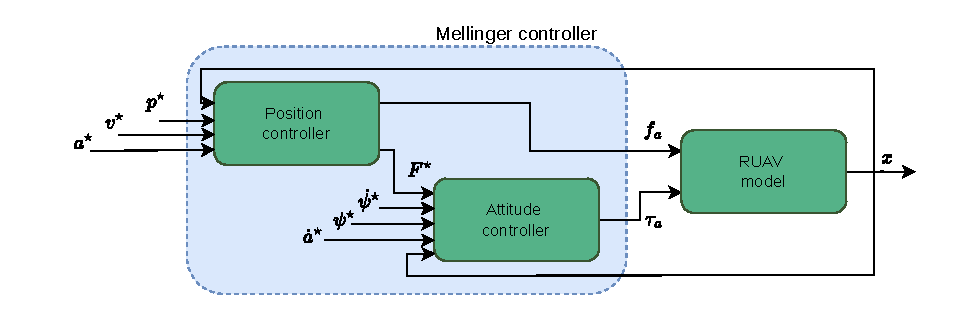
\includegraphics[width=\textwidth]{5-Figures/Chapter3/Mellinger Controller.pdf}
  \caption{NonLinear Controller architecture based in \cite{Mellinger2011}}
  \label{fig.4:mellinger_controller_architecture}
\end{figure}

\begin{figure}[htbp]
  \centering
  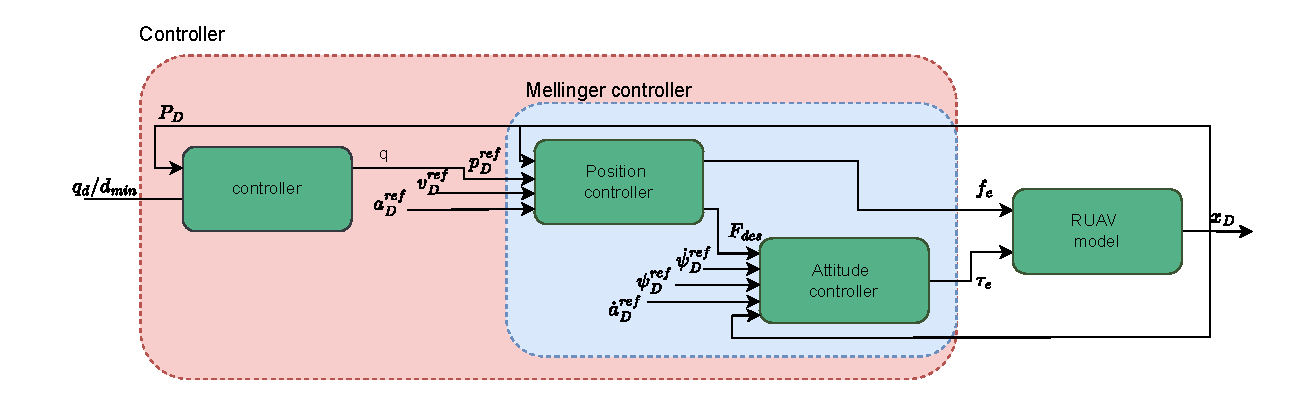
\includegraphics[width=\textwidth]{5-Figures/Chapter4/controller_architecture/generalized_controller_architecture.pdf}
  \caption{outer/inner loop controller}
  \label{fig.4:generelized_controller_architecture}
\end{figure}

\subsection{Solvers (fmincon)}

The use of numerical solvers was investigated as a means of enforcing a minimum inter-agent distance (displacement-based) while simultaneously guiding the drones toward a desired objective \gls{q_d}, defined by Fibonacci lattice points on the sphere. The optimization problem was formulated with nonlinear constraints to ensure collision avoidance.

However, this approach suffers from a fundamental limitation: none of the verified solvers is capable of enforcing all nonlinear constraints at every timestep while also guaranteeing convergence to the desired objective. The nonlinear constraints are guaranteed to be satisfied only at the optimal solution, and not throughout the system's evolution.

Figure~\ref{fig.4:solver_solution} illustrates this issue for a scenario involving three drones. It can be observed that the intermediate solver-generated trajectories do not directly converge toward the Fibonacci lattice points, highlighting the practical limitations of this approach for real-time or tightly constrained multi-agent motion planning.

\begin{figure}[htbp]
  \centering
  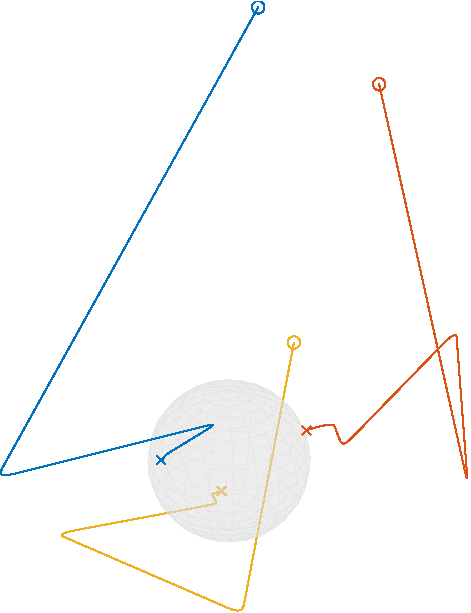
\includegraphics[width=0.4\textwidth]{5-Figures/Chapter4/solutions/solver.pdf}
  \caption{Trajectory obtained using an optimization-based solver (\texttt{fmincon}) for three drones.}
  \label{fig.4:solver_solution}
\end{figure}

\subsection{Artificial Potential Field (APF)}

Let \gls{n_D} denote the number of drones and let  
\begin{equation}
  \{ q_i^{\mathrm{fib}} \in \mathbb{S}^3 \}_{i=1}^{N_D}
\end{equation}
be the Fibonacci lattice points distributed on a sphere of radius \gls{r_s}.

The geodesic distance matrix $d_{ij}$, defined by Equation~\eqref{eq.4:geodesic_distance}, is computed between all pairs of lattice points, and the minimum safe distance \gls{d_avg} is defined as the average geodesic distance.At each simulation step \gls{k}, the position of each drone $i$ is projected onto the spherical manifold using Equation~\ref{eq.4:project_to_sphere}.

\begin{equation}
  d_{ij} =
  \begin{cases}
  r_s\arccos\!\left( \dfrac{q_i^{\top}q_j}{r_s^2} \right), & i \neq j, \\[6pt]
  \infty, & i = j .
  \end{cases}
  \label{eq.4:geodesic_distance}
\end{equation}

\begin{equation}
  d_{avg} = \frac{1}{N_D} \sum_{i=1}^{N_D} 
  \left( \frac{1}{N_D-1} \sum_{\substack{j=1 \\ j \neq i}}^{N_D} d_{ij} \right).
  \label{eq.4:d_avg between drones}
\end{equation}

\begin{equation}
  q_i(k) = r_s \frac{p_i(k)}{\|p_i(k)\|},
  \label{eq.4:project_to_sphere}
\end{equation}

where $p_i(k) \in \mathbb{R}^3$ is the Cartesian position of the drone and \gls{r_s} is the radius of the sphere. For each drone $i$, a repulsive artificial potential correction set is constructed using only neighboring drones whose geodesic distance violates the minimum safe distance constraint,
\begin{equation}
  \mathcal{N}_i(k) = \left\{ j \neq i \mid d_{ij}(k) < d_{avg} \right\}.
\end{equation}
In order words a artificial potential force is only applied if the minimal distance between drones is not satisfied. Applying both drones an equal force of opposite directions. Being the drones in the set $\mathcal{N}_i(k)$ the ones inside the minimal radius of the $i$-th drone.

The artificial potential vector applied to drone $i$ is given by
\begin{equation}
  u_i^{\mathrm{apf}}(k) =
  \sum_{j \in \mathcal{N}_i(k)}
  \left(
  q_i(k) +
  \frac{q_i(k) - q_j(k)}{\|q_i(k) - q_j(k)\|}
  \left( d_{avg} - d_{ij}(k) \right)
  \right),
\end{equation}

This basically means that the term

\begin{equation*}
  \frac{q_i(k)-q_j(k)}{\|q_i(k)-q_j(k)\|}
\end{equation*}
defines the repulsion direction from drone~$j$ to drone~$i$, while the magnitude

$\bigl(d_{avg}-d_{ij}(k)\bigr)$ increases linearly as the inter-drone distance
decreases below the minimum safety distance $d_{avg}$. To prevent excessive corrections, the vector magnitude is saturated using Equation~\eqref{eq.4:saturation_apf},meaning that the actuation of a drone at any one step never will pass the movement greater then \gls{d_avg}.

\begin{equation}
  u_i^{\mathrm{apf}}(k) \leftarrow
  \min\!\left( \|u_i^{\mathrm{apf}}(k)\|,\, d_{avg} \right)
  \frac{u_i^{\mathrm{apf}}(k)}{\|u_i^{\mathrm{apf}}(k)\|}.
  \label{eq.4:saturation_apf}
\end{equation}

Finally the resulting reference position for drone $i$ is then projected back to the sphere ensuring that all references lie on the spherical manifold.

As has been previous mentioned this reference $p^{\mathrm{ref}}(k)$ is tracked using the nonlinear Mellinger controller, which maps the desired translational accelerations and yaw angle into thrust and torque commands as has been shown in Figure~\ref{fig.4:mellinger_controller_architecture}. As a result, the drones do not converge to the original Fibonacci lattice points but instead form a dynamically generated configuration that is approximately uniformly distributed over the spherical surface while maintaining inter-agent separation. The final architecture of this method is shown in Figure~\ref{fig.4:APF_controller_architecture}, with results for 3 drones shown in Figure~\ref{fig.4:APF_solution}

\begin{figure}[htbp]
  \centering
  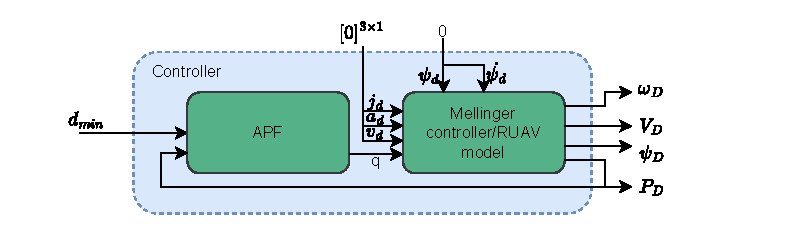
\includegraphics[width=\textwidth]{5-Figures/Chapter4/controller_architecture/APF_controller_architecture.pdf}
  \caption{outer/inner loop controller}
  \label{fig.4:APF_controller_architecture}
\end{figure}

\begin{figure}[htbp]
  \centering
  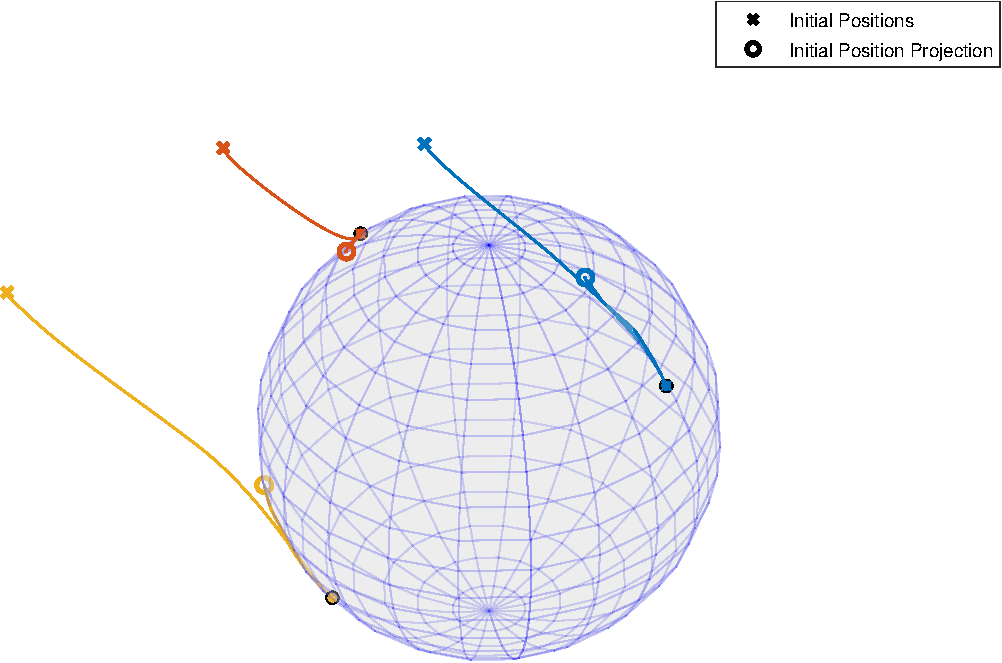
\includegraphics[width=0.8\textwidth]{5-Figures/Chapter4/solutions/APF.pdf}
  \caption{Trajectory obtained using the APF for three drones.}
  \label{fig.4:APF_solution}
\end{figure}

\subsection{Lyapunov control} \label{subsection.4:Lyapunov control}

Lyapunov controllers have been mentioned previously in Section \ref{sec.3:Lyapunov Stability and Lyapunov-Based Control}, not only the general introduction but the explicit controller to be used obtained from \cite{lyapunov_outer_loop_control}.This section describes the outer loop control architecture implementation in $\mathbb{S}^2$.

As in the \gls{APF} approach, the Fibonacci lattice is first computed as a set of reference points \(\{ q_i^{\mathrm{fib}} \in \mathbb{S}^2 \}_{i=1}^{N_D}\) distributed on a sphere of radius~\gls{r_s}.

Using the Lyapunov-based control actuation defined in Section~\ref{sec.3:Lyapunov Stability and Lyapunov-Based Control}, it is possible to retain the same inner-loop structure as the Mellinger controller used in the other methods, while redesigning the outer loop. In this formulation, the outer loop assigns a desired final position—specifically, the Fibonacci points on the sphere—and drives each drone projection \gls{q} toward its corresponding target \gls{q_d} with exponentially decreasing error.

The overall control architecture is shown in Figure~\ref{fig.4:Lyapunov_controller_architecture}, and the resulting system behavior is illustrated in Figure~\ref{fig.4:Layapunov_solution}. This formulation enables stable multi-agent motion constrained to a spherical surface while preserving geometric consistency and ensuring dynamic feasibility.

\begin{figure}[htbp]
  \centering
  \includegraphics[width=\textwidth]{5-Figures/Chapter4/controller_architecture/Lyapunov_controller_architecture.pdf}
  \caption{outer/inner loop controller}
  \label{fig.4:Lyapunov_controller_architecture}
\end{figure}

\begin{figure}[htbp]
  \centering
  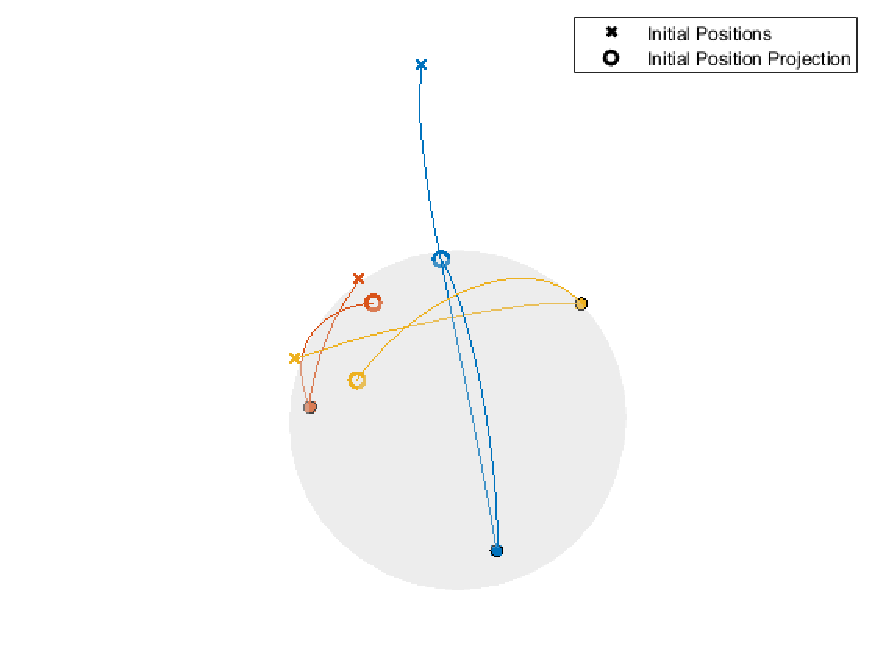
\includegraphics[width=0.8\textwidth]{5-Figures/Chapter4/solutions/lyapunov.pdf}
  \caption{Trajectory obtained using the Lyapunov for three drones.}
  \label{fig.4:Layapunov_solution}
\end{figure}

\section{Currently Optimized Implementation}

Despite the positive results obtained in Section~\ref{subsection.4:Lyapunov control} and Figure~\ref{fig.4:Layapunov_solution}, some additional improvements were introduced to the control architecture.

Instead of projecting the drone position onto a fixed two-sphere, the Fibonacci sphere points are projected onto a sphere whose radius corresponds to the current radial distance of each drone from the sphere center \gls{r}. This implies that drones starting from different initial radii will each have an associated projected Fibonacci sphere with a different radius. These radii are then gradually reduced toward the desired sphere radius according to the gain $K_{\mathrm{rad}}$, as defined in the radial update law in Equation~ \ref{eq.4:radius_update}.

\begin{equation}
\begin{aligned}
    q_s &= q - c_{\text{sphere}}, \\
    \dot{r} &= K_{\mathrm{rad}} \cdot \frac{1}{2}
    \left(1 + \frac{q_s^\top q_d}{\|q_s\|\,\|q_d\|}\right)
    \left(R_s - r\right), \\
    r_{k+1} &= r_k + \Delta t\, \dot{r},
\end{aligned}
\label{eq.4:radius_update}
\end{equation}
Where $c_{\text{sphere}}$ the center of the sphere, and $r$ is the current radius of the projected sphere, \gls{r_s} is the desired final sphere radius, and $\Delta t$ is the simulation sampling period. In Figure~\ref{fig.4:Layapunov_solution_explained} its possible to better visualize this improvement made where the fibonacci points, "Final Objective" is projected to the current radius of the drone \gls{q_d} being the \gls{q} the currently desired point for the drone \gls{p_D_ref}.

Another improvement was made where instead of moving toward a randomly selected Fibonacci point on the sphere, the drones are assigned to target points using the Munkres algorithm. Given a cost matrix defined as the geodesic distance between each drone and all target points projected onto the final-radius sphere \gls{r_s}, the algorithm computes an optimal solution to the \gls{GNN} assignment problem. This solution minimizes the total assignment cost. No custom implementation of the algorithm was developed; instead, the built-in \(\text{MATLAB}^\text{\textregistered}\) \cite{MATLAB:R2024a} function \textit{assignmunkres} \cite{MATLAB_assignmunkres} was used.

\begin{figure}[htbp]
  \centering
  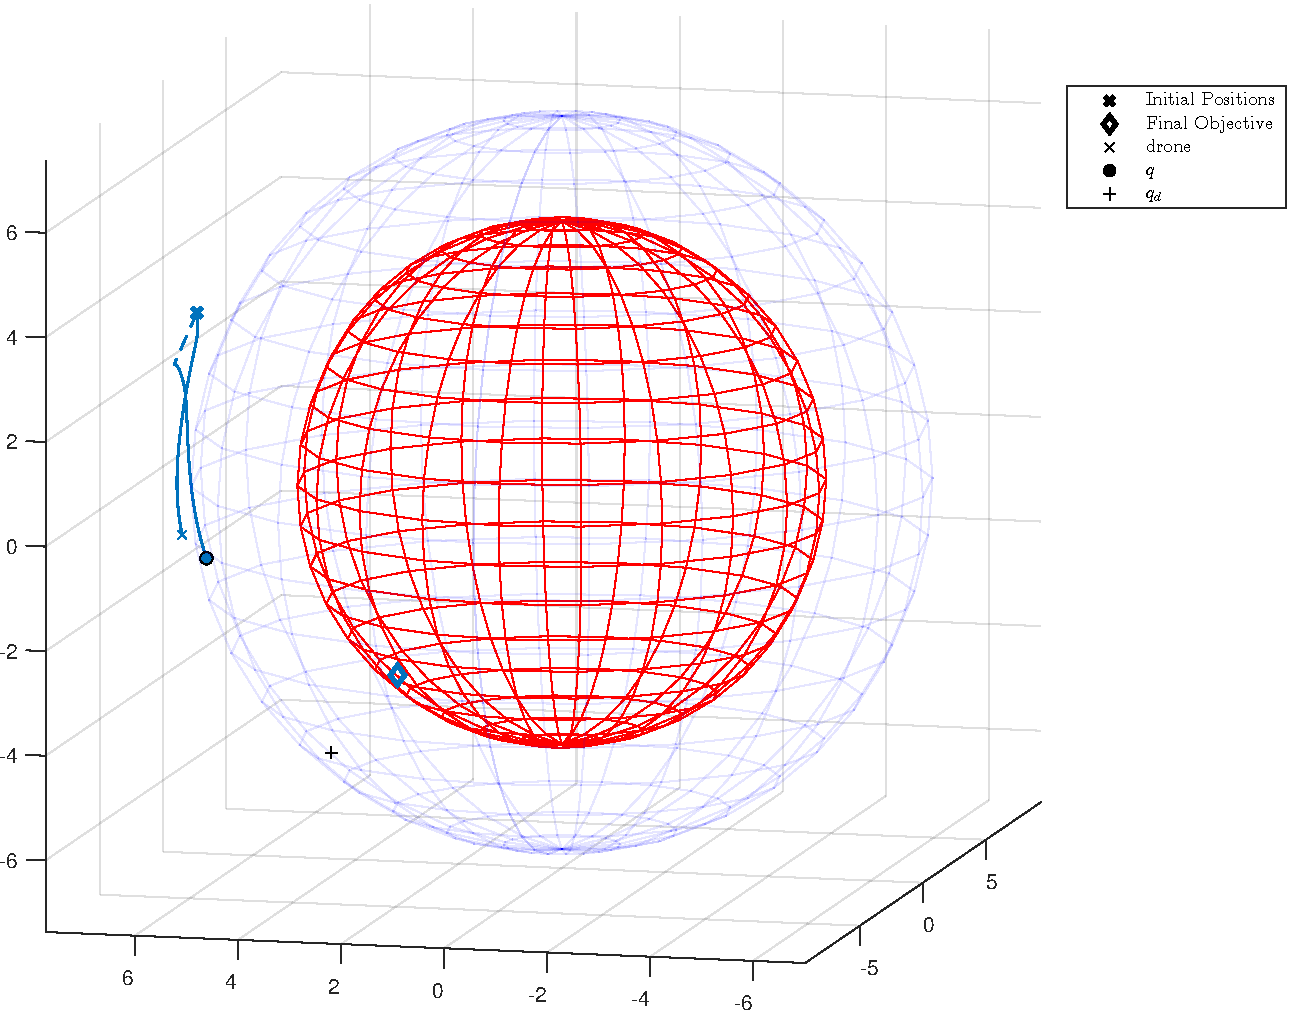
\includegraphics[width=0.8\textwidth]{5-Figures/Chapter4/solutions/final_result_explained.pdf}
  \caption{Trajectory obtained for 1 drone mid simulation.}
  \label{fig.4:Layapunov_solution_explained}
\end{figure}

\subsection{Simulation Setup}

The simulation was performed using the parameters listed below.

\begin{table}[h]
\centering
\caption{General simulation parameters.}
\begin{tabular}{l c}
\hline
Parameter & Value \\
\hline
Simulation duration $T_{\text{end}}$ & $15~\text{s}$ \\
Sampling period $\Delta t$ & $0.01~\text{s}$ \\
Gravity \gls{g} & $9.81~\text{m/s}^2$ \\
Number of drones \gls{n_D} & $3$ \\
Desired sphere radius \gls{r_s} & $5~\text{m}$ \\
Radial gain $K_{\mathrm{rad}}$ & $0.3$ \\
\hline
\end{tabular}
\end{table}

\begin{table}[h]
\centering
\caption{Outer-loop control parameters.}
\begin{tabular}{l c}
\hline
Parameter & Value \\
\hline
Damping coefficient $c$ & $0.3$ \\
Inertia matrix \gls{I_q} &
$\mathrm{diag}(0.0294,\;0.0305,\;0.0495)$ \\
Additional torques $\tau$ & $\mathbf{0}_{3\times1}$ \\
Position gain $K_r$ & $\mathrm{diag}(70,\;70,\;70)$ \\
Angular velocity gain $K_\omega$ &
$10^{-1}\,\mathrm{diag}(7.056,\;7.320,\;11.88)$ \\
\hline
\end{tabular}
\end{table}

\begin{table}[h]
\centering
\caption{Inner-loop control parameters.}
\begin{tabular}{l c}
\hline
Parameter & Value \\
\hline
Mass \gls{m_D} & $5~\text{kg}$ \\
Inertia matrix \gls{I_D} &
$\mathrm{diag}(0.02,\;0.02,\;0.03)$ \\
Drag coefficient $D$ & $0$ \\
Proportional gain $K_p$ & $\mathrm{diag}(150,\;150,\;150)$ \\
Velocity gain $K_v$ & $\mathrm{diag}(15,\;15,\;15)$ \\
Integral gain $K_i$ & $\mathbf{0}_{3\times3}$ \\
Attitude gain $K_R$ & $\mathrm{diag}(8,\;8,\;8)$ \\
Angular rate gain $K_\Omega$ & $\mathrm{diag}(0.5,\;0.5,\;0.5)$ \\
\hline
\end{tabular}
\end{table}

Being the initial angular coordinates and radii of the drones given by and recalculated to cartesian using equation~\eqref{eq.4:spherical_to_cartesian}.

\begin{align*}
    \theta_0 &= [0.175,\;0.698,\;1.222], \\
    \phi_0 &= [1.484,\;1.222,\;1.396], \\
    r_0 &= [13,\;15,\;11].
\end{align*}

\begin{equation}
    q_0 = r_0
    \begin{bmatrix}
        \sin\theta_0 \cos\phi_0 \\
        \sin\theta_0 \sin\phi_0 \\
        \cos\theta_0
    \end{bmatrix}.
    \label{eq.4:spherical_to_cartesian}
\end{equation}

\subsubsection{Target Motion}

The target $T_{pos}$ trajectory is defined as the following piecewise function:
\begin{equation*}
  T_{pos} =
  \begin{cases}
  \begin{bmatrix}
  3t &
  0 &
  0
  \end{bmatrix}^\top,
  & t \le 1.5 \\[8pt]

  \begin{bmatrix}
  3t &
  -3(t - 1.5) &
  0
  \end{bmatrix}^\top,
  & 1.5 < t \le 3 \\[8pt]

  \begin{bmatrix}
  9 &
  -4.5 &
  0
  \end{bmatrix}^\top,
  & t > 3
  \end{cases}
\end{equation*}

In Figure~\ref{fig.4:Lyapunov_solution_final} the final result obtained with the improvements above mentioned can be visualized. As it is possible to see the chaser drones are capable of encircling the target even if the same is in motion, note that as mentioned in \cite{Mycielski1988} the chasers must at least have the same velocity as the target to be able to achieve this results. 

\begin{figure}[htbp]
  \centering

  % --- Top row (2 figures) ---
  \subfloat[$t=0$]{%
    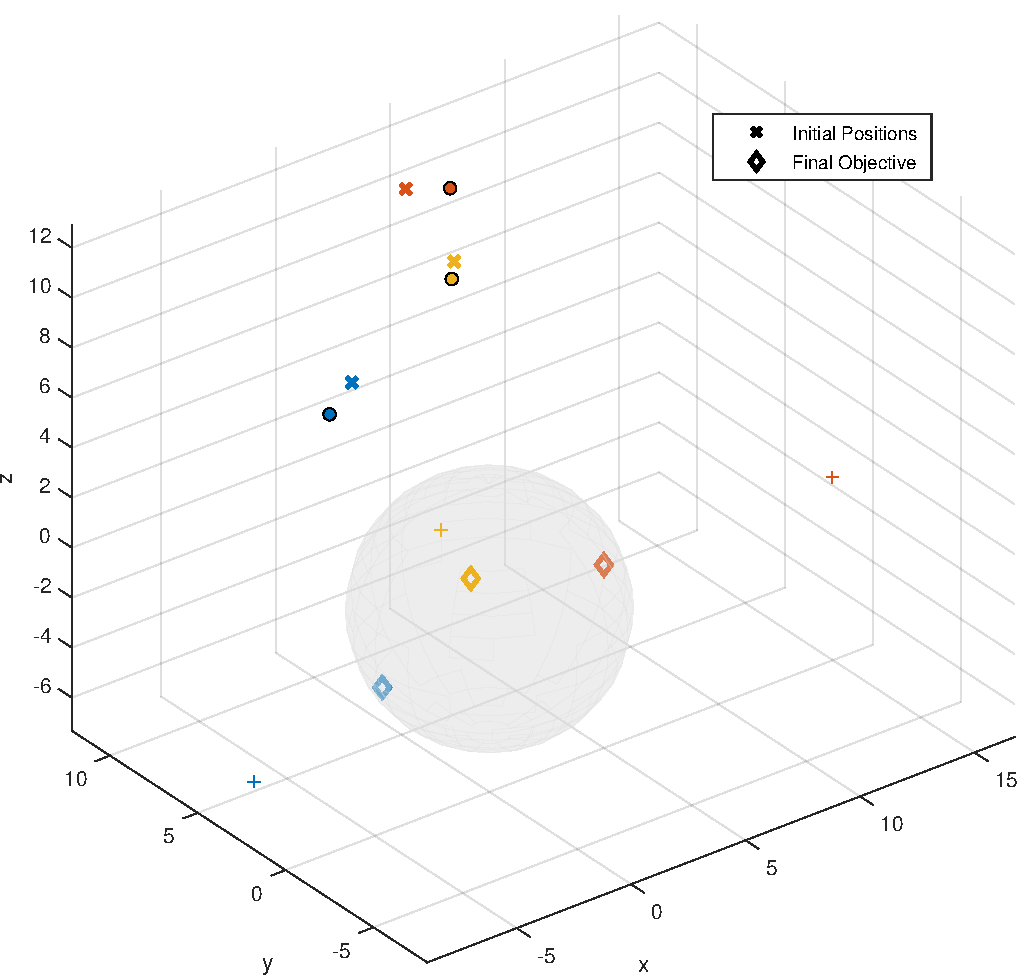
\includegraphics[width=0.45\textwidth]{5-Figures/Chapter4/solutions/final_result_t_0.pdf}
  }\hfill
  \subfloat[$t=3$]{%
    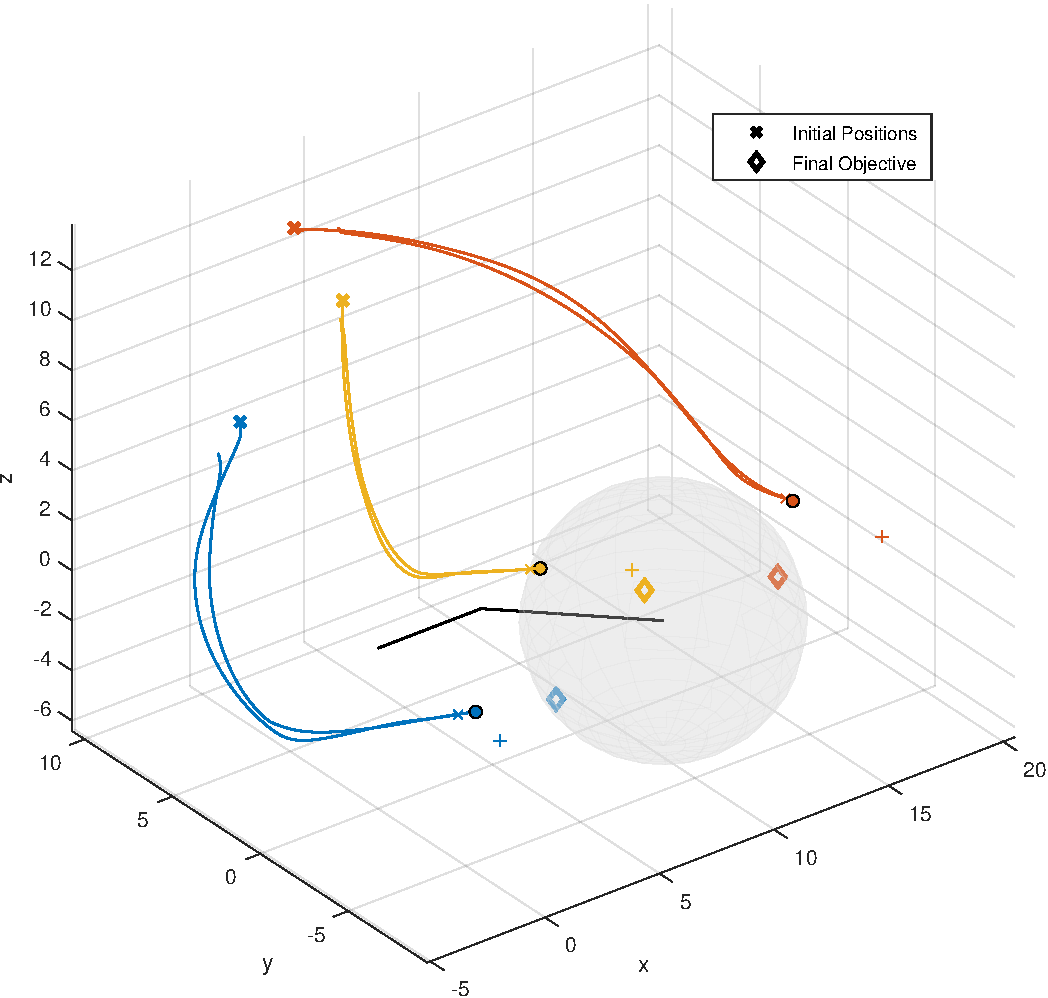
\includegraphics[width=0.45\textwidth]{5-Figures/Chapter4/solutions/final_result_t_3.pdf}
  }

  \vspace{0.5cm}

  % --- Bottom row (1 centered figure) ---
  \subfloat[$t=15$]{%
    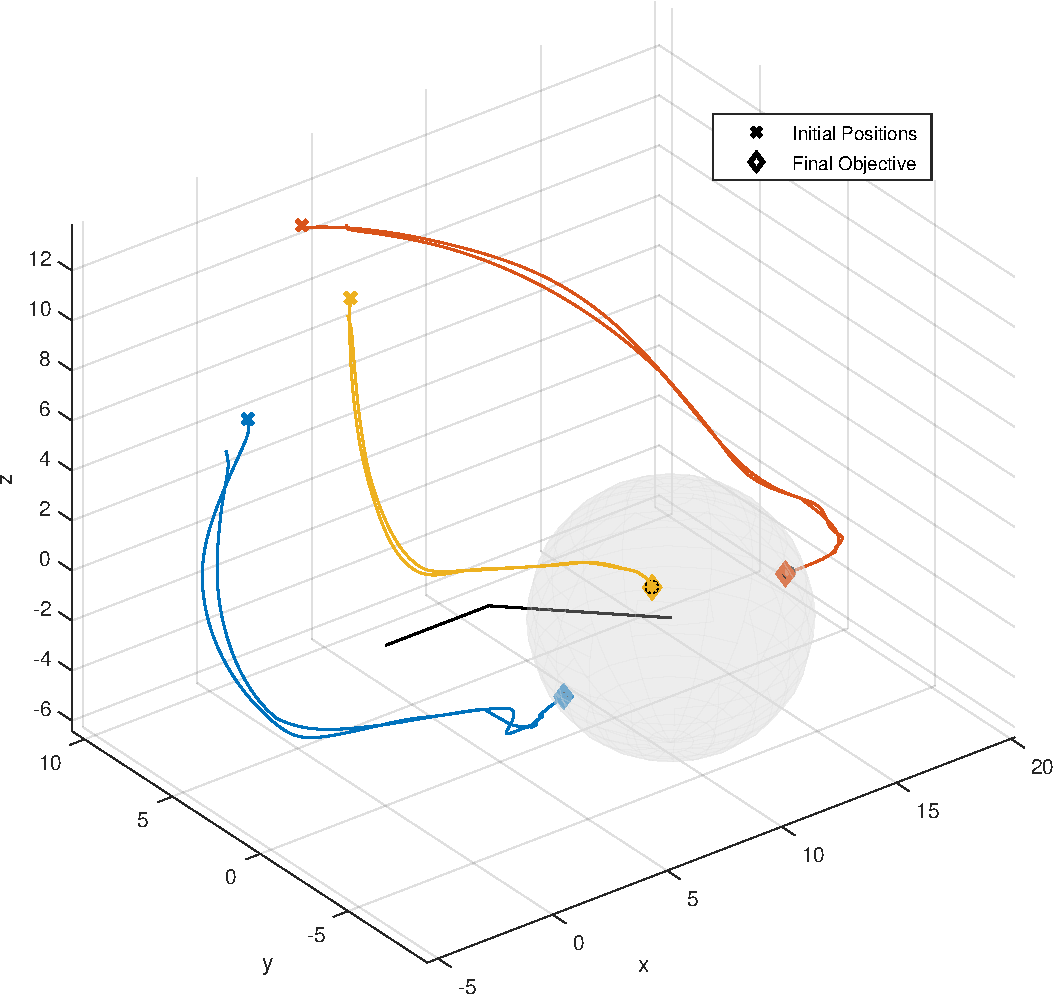
\includegraphics[width=0.45\textwidth]{5-Figures/Chapter4/solutions/final_result_t_15.pdf}
  }

  \caption{Trajectory obtained using the Lyapunov for three drones. ($t$ in seconds)}
  \label{fig.4:Lyapunov_solution_final}
\end{figure}

\section{Safe Guard methods} \label{sec.5:Safe Guard methods}
Despite having a trajectory from the chasers to their respective final desired position no guarantee about collision avoidance is given, in this section that exact subject is discussed, two main methods will be discussed \gls{APF}, \gls{CBF} or \gls{HOCBF}. To introduce more formally the subject it will be first \gls{APF} since they are the simpler of the presented methods.

\subsection{Artificial Potential Fields}
\gls{APF} have been introduced previously at \ref{sec.4:Control loop architecture}

The safeguard operates directly on the spherical manifold
$\Gamma^2$ and modifies only the reference position ${q}_i$, preserving the
nonlinear controller stability and the Lyapunov controller convergence structure.
Specifically, at each control step, the current UAV positions are
projected onto the sphere of radius $r^\star$ centered at the target
\begin{equation}
    q_{i}^{r^\star} = \Pi_{\Gamma^2}^{r^\star,p_T}(\dot{q}_i)
\end{equation}

Pairwise geodesic distances on $\Gamma^2$ are then computed.
Let $d_{ij}$ denote the spherical geodesic distance between UAVs $i$
and $j$. A minimum safe separation $d_{\min} > 0$ is defined, in this case half of the the average geodesic distance between the fibonacci points $p^\star$ is used.
For each neighboring UAV satisfying $d_{ij} < d_{\min}$, a repulsive
tangential displacement is generated.

Let
\begin{equation}
    n_i = \frac{q_{i}^{r^\star} - p_T}{\|q_{i}^{r^\star} - p_T\|}
\end{equation}
denote the outward normal direction at UAV $i$.
The relative displacement vector
\begin{equation}
    \Delta_{ij} = q_{i}^{r^\star} - q_{j}^{\mathrm{proj}}
\end{equation}
is decomposed into radial and tangential components.
Only the tangential component
\begin{equation}
    \Delta_{ij}^{\top}
    =
    \Delta_{ij}
    -
    (\Delta_{ij}^{\top} n_i) n_i
\end{equation}
is retained, ensuring that the safeguard does not interfere with
radial stabilization.

The repulsive contribution from agent $j$ to agent $i$ is defined as
\begin{equation}
    f_{ij}
    =
    (d_{\min} - d_{ij})
    \frac{\Delta_{ij}^{\top}}{\|\Delta_{ij}^{\top}\|},
    \quad d_{ij} < d_{\min},
\end{equation}
The total artificial potential displacement is obtained by summing all
active pairwise contributions
\begin{equation}
    f_i = \sum_{j \neq i} f_{ij}.
\end{equation}

To prevent excessive deviation from the nominal reference, the
resulting displacement is saturated to a bounded magnitude of a maximum of $d_{min}$ and the
corrected reference is re-projected onto the sphere:
\begin{equation}
    \tilde{q}_i =
    \Pi_{\Gamma^2}^{r_i,p_T}
    \left(
        q_{i}^{r^\star} + f_i
    \right),
    \label{eq:apf_result}
\end{equation}
The safeguard therefore produces a modified reference direction
$\tilde{q}_i$ that maintains spherical consistency while enforcing
minimum separation during transients.

\paragraph*{Stability Discussion}

The APF term acts as a bounded perturbation to the nominal
reduced-attitude reference. Since the artificial potential vanishes
whenever $d_{ij} \ge d_{\min}$ for all $j$, the nominal equilibrium
configuration remains unchanged. Furthermore, because the perturbation
is tangential and bounded, the almost-global asymptotic stability of
the reduced-attitude equilibrium is preserved in the sense of
input-to-state stability with respect to the safeguard perturbation.

In practice, this mechanism alleviates collision avoidance during
convergence while allowing the Lyapunov-based controller to recover
the desired encirclement configuration once agents are safely
separated. But it cannot guarantee collision avoidance unlike the \gls{CBF} which does guarantee.

\subsection{Control Barrier Functions}
